\documentclass{beamer}


% Setup appearance:

\usetheme{Darmstadt}
\usefonttheme[onlylarge]{structurebold}
\setbeamerfont*{frametitle}{size=\normalsize, series=\bfseries}
\setbeamertemplate{navigation symbols}{}


% Standard packages

\usepackage[english]{babel}
\usepackage[latin1]{inputenc}
\usepackage{times}
\usepackage[T1]{fontenc}
\usepackage{hyperref}

% Setup TikZ

\usepackage{ifthenx}
\usepackage{tikz}
\usetikzlibrary{arrows}
\usetikzlibrary{calc}
\usepackage{pgfmath}
\usepackage{verbatim}
\usepackage{listings}
\usepackage{ulem}
\tikzstyle{block}=[draw opacity=0.7, line width=1.4cm]
\lstset{language=C}

% Author, Title, etc.

\title[Anomaly Detection System Overview]
{%
Stocks project
%
}

\author[Sinha N]
{
  Nish~Sinha\inst{1} \and
}

\institute[Xad]
{
  \inst{1}%
  Nsinha Inc.,  CA, USA
  \and
  \vskip-2mm
}

\date[\today]
{\today}



% The main document
\newcommand{\drawBoxVertText}[5]{{0}
		\shade[top color=#4, bottom color=#4,xslant=#5] (#1) rectangle (#2) node[midway,below][label={[rotate=-90]left:#3}] {};

%node[midway][above] [label={[rotate=-90]above:#3}]{};
}

\newcommand {\drawArrowLToRAbove}[3] {
	\draw[->, auto] let
		\p1 = (#1), \p2 = (#2)
		in
		(\x1  ,\y1) -- (\x2,\y2)  
		(\x1  ,\y1) -- (\x2,\y2)  node[midway][above] {#3};
}

\newcommand{\drawLinkArrowVertical}[4]{
	\draw[->, auto] let
		\p1 = (#1), \p2 = (#2),
		\p3 = (#3), \p4 = (#4)
		in
		({(\x1 + \x2)*1/2} ,\y1) -- ({(\x3 + \x4)*1/2} ,\y4);
}

\newcommand{\drawLinkArrowVerticalWithOffset}[4]{
	\draw[->, auto] let
		\p1 = (#1), \p2 = (#2),
		\p3 = (#3), \p4 = (#4)
		in
		(\x1  ,\y1) -- (\x3 ,\y4);
}
\newcommand{\drawLinkArrowHorizontal}[4]{
	\draw[<->] let
		\p1 = (#1), \p2 = (#2),
		\p3 = (#3), \p4 = (#4)
		in
		(\x2, {(\y1 + \y2)*1/2}) -- (\x3, {(\y3 + \y4)*1/2});
}

\newcommand{\drawBox}[5]{{0}
		\shade[top color=#4, bottom color=#4,xslant=#5] (#1) rectangle (#2) node[midway,below] {#3};
}

\newcommand{\drawBoxTextBottom}[7]{{0}
		\shade[top color=#4, bottom color=#4,xslant=#5] (#1) rectangle (#2) node[left=#6in,below=#7in] {#3};
}

\begin{document}

\begin{frame}
  \titlepage
\end{frame}



\section{The Design}

\subsection{Flow Diagram }

\begin{frame}{data structure}

    \begin{itemize}
	\item Think of data of all stocks as json file
	\item each data point belongs to a given stock and ex
    		\begin{itemize}
			\item may contain time zone(utc implicit)
			\item current value at instant
			\item instant time stamp with tags like local,unix,utc,precision
			\item current volume at instant(normally this is day's volume from start of day.
			\item high ,low price
			\item open price and day's start timestamap(us start time only)
			\item day's end timestamp(us end time)
			\item previous working day's start timestamp ,end ts, volume, price,high ,low,open,close,percent change
		\end{itemize}
	\item each attribute has a default start at day. Volume starts with 0.Price starts with last closing price(in case available or current price if not available). Data structure should have this notion when storing. 
	\item a compendium of above data will make a total world. 
	
	\end{itemize}
	
\end{frame}

\begin{frame}{ops on data}

	\begin{itemize}
		\item find the graph on a given dimension
		\item sort data as per time stamp and project attributes 
		\item create csv files on any set of attributes and study it.
	\end{itemize}
\end{frame}


\begin{frame}{simplification}
	\begin{itemize}
		\item days data instead of hourly data
	
	\end{itemize}
\end{frame}

\begin{frame}{Rough implementation flow}
	\begin{itemize}
		\item we ingest a day's data.
		\item we append to an aggergate yearly file and corresponding entry meta file. Metafile is for deduplication.
		\item We can assume we have year loads of files containg day's data for years in past and current. The current year is still getting loaded.

		\item We can analyze these files for specific stock dumps. like dumping the flow data and analyzing it in python etc.
	
	\end{itemize}
\end{frame}


\begin{frame}
	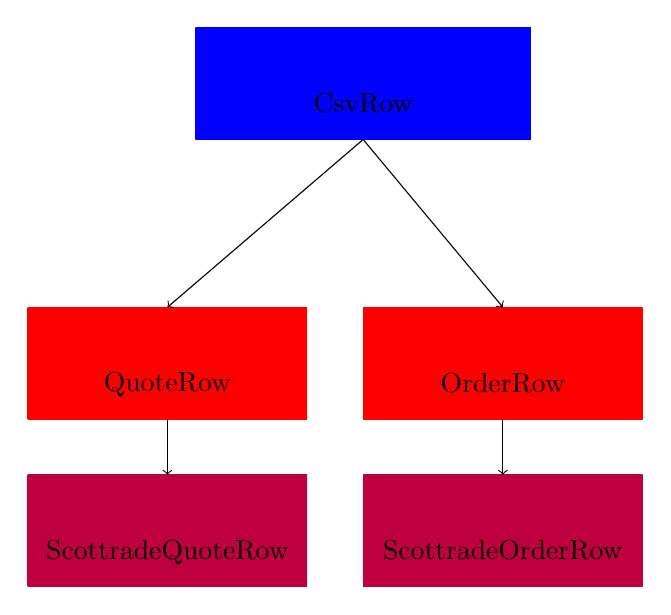
\begin{tikzpicture}[scale=0.71]

		\coordinate (B1_L) at (0,0);
		\coordinate (B1_R) at (5,2);
		\coordinate (B2_L) at (6,0);
		\coordinate (B2_R) at (11,2);
		\coordinate (B3_L) at (3,5);
		\coordinate (B3_R) at (9,7);
		\coordinate (B4_L) at (0,-3);
		\coordinate (B4_R) at (5,-1);
		\coordinate (B5_L) at (6,-3);
		\coordinate (B5_R) at (11,-1);

		\drawBox{B1_L}{B1_R}{QuoteRow}{red}{0}
		\drawBox{B2_L}{B2_R}{OrderRow}{red}{0}
		\drawBox{B3_L}{B3_R}{CsvRow}{blue}{0}
		\drawBox{B4_L}{B4_R}{ScottradeQuoteRow}{purple}{0}
		\drawBox{B5_L}{B5_R}{ScottradeOrderRow}{purple}{0}
		\drawLinkArrowVertical {B3_L}{B3_R}{B1_L}{B1_R}
		\drawLinkArrowVertical {B3_L}{B3_R}{B2_L}{B2_R}
		\drawLinkArrowVertical {B1_L}{B1_R}{B4_L}{B4_R}
		\drawLinkArrowVertical {B2_L}{B2_R}{B5_L}{B5_R}

	\end{tikzpicture}
\end{frame}

\begin{frame}
	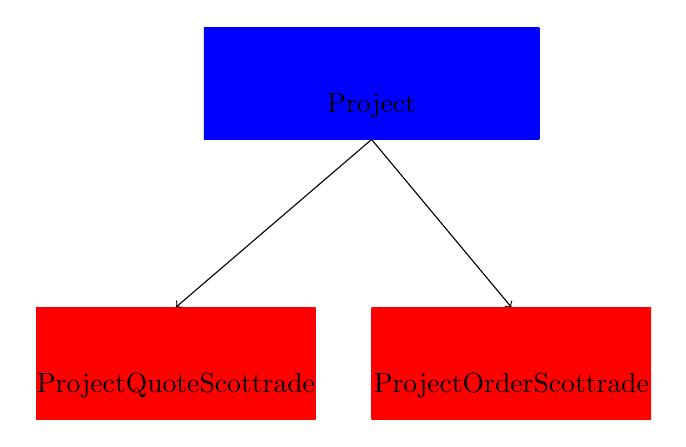
\begin{tikzpicture}[scale=0.71]
		\coordinate (B1_L) at (0,0);
		\coordinate (B1_R) at (5,2);
		\coordinate (B2_L) at (6,0);
		\coordinate (B2_R) at (11,2);
		\coordinate (B3_L) at (3,5);
		\coordinate (B3_R) at (9,7);

		\drawBox{B1_L}{B1_R}{ProjectQuoteScottrade}{red}{0}
		\drawBox{B2_L}{B2_R}{ProjectOrderScottrade}{red}{0}
		\drawBox{B3_L}{B3_R}{Project}{blue}{0}
		\drawLinkArrowVertical {B3_L}{B3_R}{B1_L}{B1_R}
		\drawLinkArrowVertical {B3_L}{B3_R}{B2_L}{B2_R}

	\end{tikzpicture}
\end{frame}




\begin{frame}
   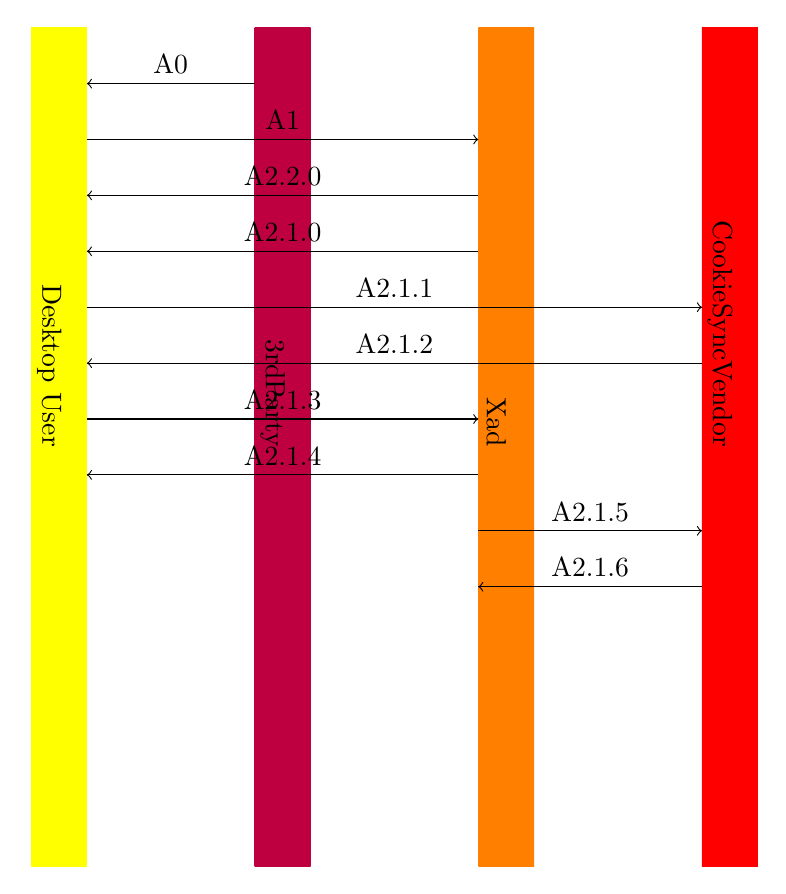
\begin{tikzpicture}[scale=0.71]
	\coordinate (B1_L) at (0,0);
	\coordinate (B1_R) at (1,15);
	\coordinate (B2_L) at (4,0);
	\coordinate (B2_R) at (5,15);
	\coordinate (B3_L) at (8,0);
	\coordinate (B3_R) at (9,15);
	\coordinate (B4_L) at (12,0);
	\coordinate (B4_R) at (13,15);

	\coordinate (AR0_L) at (4,14);
	\coordinate (AR0_R) at (1,14);
	\coordinate (AR1_L) at (1,13);
	\coordinate (AR1_R) at (8,13);
	\coordinate (AR2_L) at (8,12);
	\coordinate (AR2_R) at (1,12);
	\coordinate (AR3_L) at (8,11);
	\coordinate (AR3_R) at (1,11);
	\coordinate (AR4_L) at (1,10);
	\coordinate (AR4_R) at (12,10);
	\coordinate (AR5_L) at (12,9);
	\coordinate (AR5_R) at (1,9);
	\coordinate (AR6_L) at (1,8);
	\coordinate (AR6_R) at (8,8);
	\coordinate (AR7_L) at (8,7);
	\coordinate (AR7_R) at (1,7);
	\coordinate (AR8_L) at (8,6);
	\coordinate (AR8_R) at (12,6);
	\coordinate (AR9_L) at (12,5);
	\coordinate (AR9_R) at (8,5);
	
	\drawBoxVertText{B1_L}{B1_R}{Desktop User}{yellow}{0}
	\drawBoxVertText{B2_L}{B2_R}{3rdParty}{purple}{0}
	\drawBoxVertText{B3_L}{B3_R}{Xad}{orange}{0}
	\drawBoxVertText{B4_L}{B4_R}{CookieSyncVendor}{red}{0}
	\drawArrowLToRAbove{AR0_L}{AR0_R}{A0}
	\drawArrowLToRAbove{AR1_L}{AR1_R}{A1}
	\drawArrowLToRAbove{AR2_L}{AR2_R}{A2.2.0}
	\drawArrowLToRAbove{AR3_L}{AR3_R}{A2.1.0}
	\drawArrowLToRAbove{AR4_L}{AR4_R}{A2.1.1}
	\drawArrowLToRAbove{AR5_L}{AR5_R}{A2.1.2}
	\drawArrowLToRAbove{AR6_L}{AR6_R}{A2.1.3}
	\drawArrowLToRAbove{AR7_L}{AR7_R}{A2.1.4}
	\drawArrowLToRAbove{AR8_L}{AR8_R}{A2.1.5}
	\drawArrowLToRAbove{AR9_L}{AR9_R}{A2.1.6}

  \end{tikzpicture}
\end{frame}




\subsection{Flow Diagram }
\begin{frame}[fragile]{Transition Flow Diagram pattern A-1}
    \tiny
    \begin{itemize}
        \item  \textbf{A0:} da da da
	\alert {TIMESTAMP macro should be supported by our accounts}
	\url{http://google.api.com}\\
	\url{redirect=}\\
   \end{itemize}
\end{frame}



\end{document}

